\chapter{\texorpdfstring{BPMN Analysis}{BPMN Analysis}}
\label{ch:16b}
\lecturemeta{Lezione 16b \quad\textbullet\quad 2026-07-04 \quad\textbullet\quad Roberto Bruni}{Weske, \emph{Business Process Management}, Ch.5.7}

Dopo aver dato semantica formale agli \hyperref[ch:16a]{EPC}, facciamo lo stesso con il \textbf{BPMN} (visto in \hyperref[ch:07a]{07a — EPC e BPMN} e \hyperref[ch:07b]{07b — More BPMN}). Il programma è identico: tradurre il diagramma in un net e dichiararlo \emph{sound} se il net lo è. Ma ci sono due novità importanti — un "twist" nella traduzione, e il fatto che il BPMN gestisce anche le \textbf{collaboration}, che si traducono in \textbf{workflow system} (più process che comunicano).

\begin{boxabstract}{Il piano}
\begin{itemize}
\item I \textbf{BPMN process diagram} si traducono in \textbf{workflow net} $\rightarrow$ si verifica la soundness con gli strumenti soliti (liveness + boundedness di $N^\star$).
\item I \textbf{BPMN collaboration diagram} si traducono in \textbf{workflow system} (più net che si scambiano messaggi).
\item Un diagramma BPMN è \textbf{sound} se il suo net/system è sound.
\end{itemize}

Come per gli EPC, le difficoltà maggiori vengono dagli \textbf{OR-gateway}: la raccomandazione pratica è \textbf{evitarli} (tutti i problemi visti con gli EPC valgono identici anche qui).
\end{boxabstract}

Va detto che dare una semantica formale al BPMN è stato oggetto di \textbf{molti tentativi} (Abstract State Machines, term/graph rewriting, process algebra, temporal logic, …): noi seguiamo la via dei Petri net (Dijkman, Dumas, Ouyang, 2008).

\section{\texorpdfstring{Richiamo: BPMN vs EPC}{Richiamo: BPMN vs EPC}}

I due linguaggi hanno elementi in corrispondenza abbastanza diretta, con in più le \textbf{swimlane} (pool e lane) e il \textbf{message flow}, che nel BPMN servono a modellare la comunicazione fra partecipanti.

\begin{figure}[!htb]
\centering
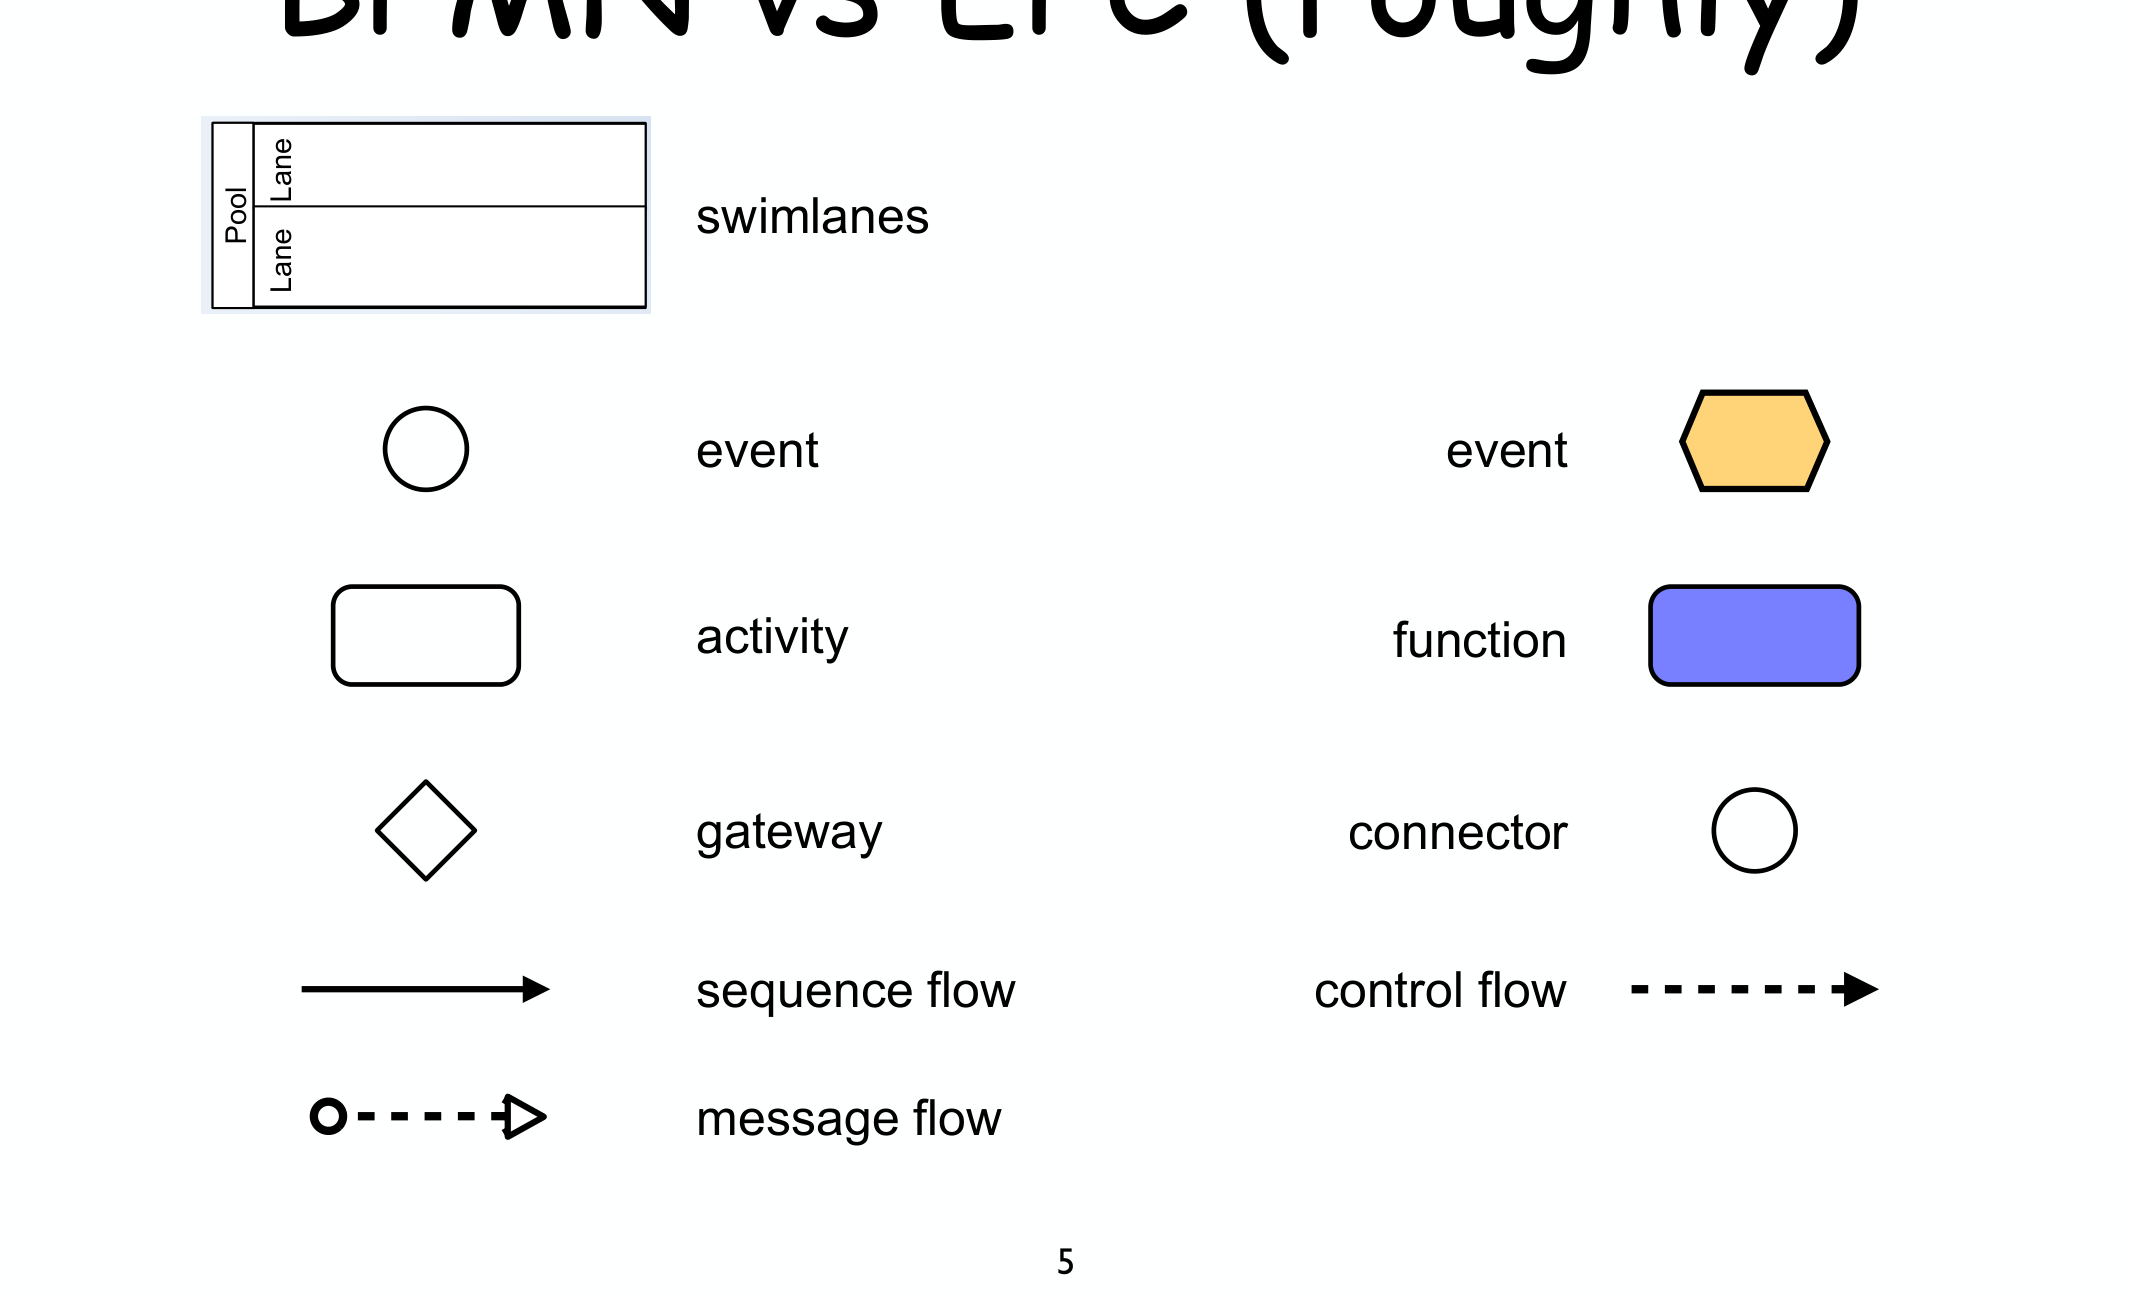
\includegraphics[width=0.74\linewidth,height=0.34\textheight,keepaspectratio]{images/16b-bpmn-analysis_p4_bpmn-vs-epc.png}
\caption{BPMN vs EPC "roughly": activity $\leftrightarrow$ function, gateway $\leftrightarrow$ connector, sequence flow $\leftrightarrow$ control flow. In più il BPMN ha \textbf{swimlane} (pool/lane) e \textbf{message flow} per la comunicazione fra partecipanti.}
\end{figure}

\section{\texorpdfstring{La semplificazione dei diagrammi}{La semplificazione dei diagrammi}}

Come per gli EPC, ci si restringe a una classe "ben formata" di diagrammi, i \textbf{simplified BPMN}, per rendere la traduzione uniforme.

\begin{boxdefinition}{Simplified BPMN}
\begin{itemize}
\item uno \textbf{start / exception event} ha \textbf{un solo} flusso uscente e \textbf{nessuno} entrante;
\item un \textbf{end event} ha \textbf{un solo} flusso entrante e \textbf{nessuno} uscente;
\item tutte le \textbf{activity} e gli \textbf{intermediate event} hanno \textbf{esattamente un} flusso entrante e \textbf{uno} uscente;
\item ogni \textbf{gateway} ha \emph{o} un flusso entrante (e più uscenti), \emph{o} un flusso uscente (e più entranti) — mai molti-a-molti.
\end{itemize}
\end{boxdefinition}

Questi vincoli \textbf{non sono una vera limitazione}: qualsiasi diagramma si può normalizzare con piccole trasformazioni meccaniche (un "desugaring").

\begin{boxnote}{Come normalizzare (desugar)}
\begin{itemize}
\item elemento con \textbf{più flussi entranti} $\rightarrow$ si inserisce prima un \textbf{XOR-join};
\item elemento con \textbf{più flussi uscenti} $\rightarrow$ si inserisce dopo un \textbf{AND-split};
\item gateway \textbf{molti-a-molti} $\rightarrow$ si \textbf{decompone in due} gateway (uno join, uno split);
\item si aggiungono start/end event dove mancano.
\end{itemize}

Restano fuori: \textbf{OR-gateway} (da evitare), forme limitate di sub-processing, niente transaction né compensation.
\end{boxnote}

\section{\texorpdfstring{Il "twist" della traduzione}{Il "twist" della traduzione}}

Ed ecco la sorpresa. Negli EPC la corrispondenza era: event $\rightarrow$ \textbf{place}, function $\rightarrow$ \textbf{transition}, arco $\rightarrow$ arco. Nel BPMN è \textbf{diversa}, e a prima vista controintuitiva:

\begin{boxwarning}{The twist! (attenzione, è diverso dagli EPC)}
\begingroup\small
\begin{tabularx}{\linewidth}{>{\raggedright\arraybackslash}X>{\raggedright\arraybackslash}X}
\toprule
\textbf{Oggetto BPMN} & \textbf{Frammento di net} \\
\midrule
\textbf{event} & \textbf{transition} \\
\textbf{activity} & \textbf{transition} \\
\textbf{sequence flow} / \textbf{message flow} & \textbf{place} \\
\bottomrule
\end{tabularx}
\endgroup

Cioè: \textbf{sia gli event sia le activity diventano transition}, e sono gli \textbf{archi} (i flussi) a diventare \textbf{place}! È il contrario dell'intuizione EPC, dove erano gli eventi a diventare place.
\end{boxwarning}

Il motivo è che nel BPMN un event è un \emph{accadimento istantaneo} (come uno scatto di transition), mentre lo "stato" del processo è catturato dal \emph{flusso} in cui si trova il token — quindi sono gli archi a fare da place.

\begin{figure}[!htb]
\centering
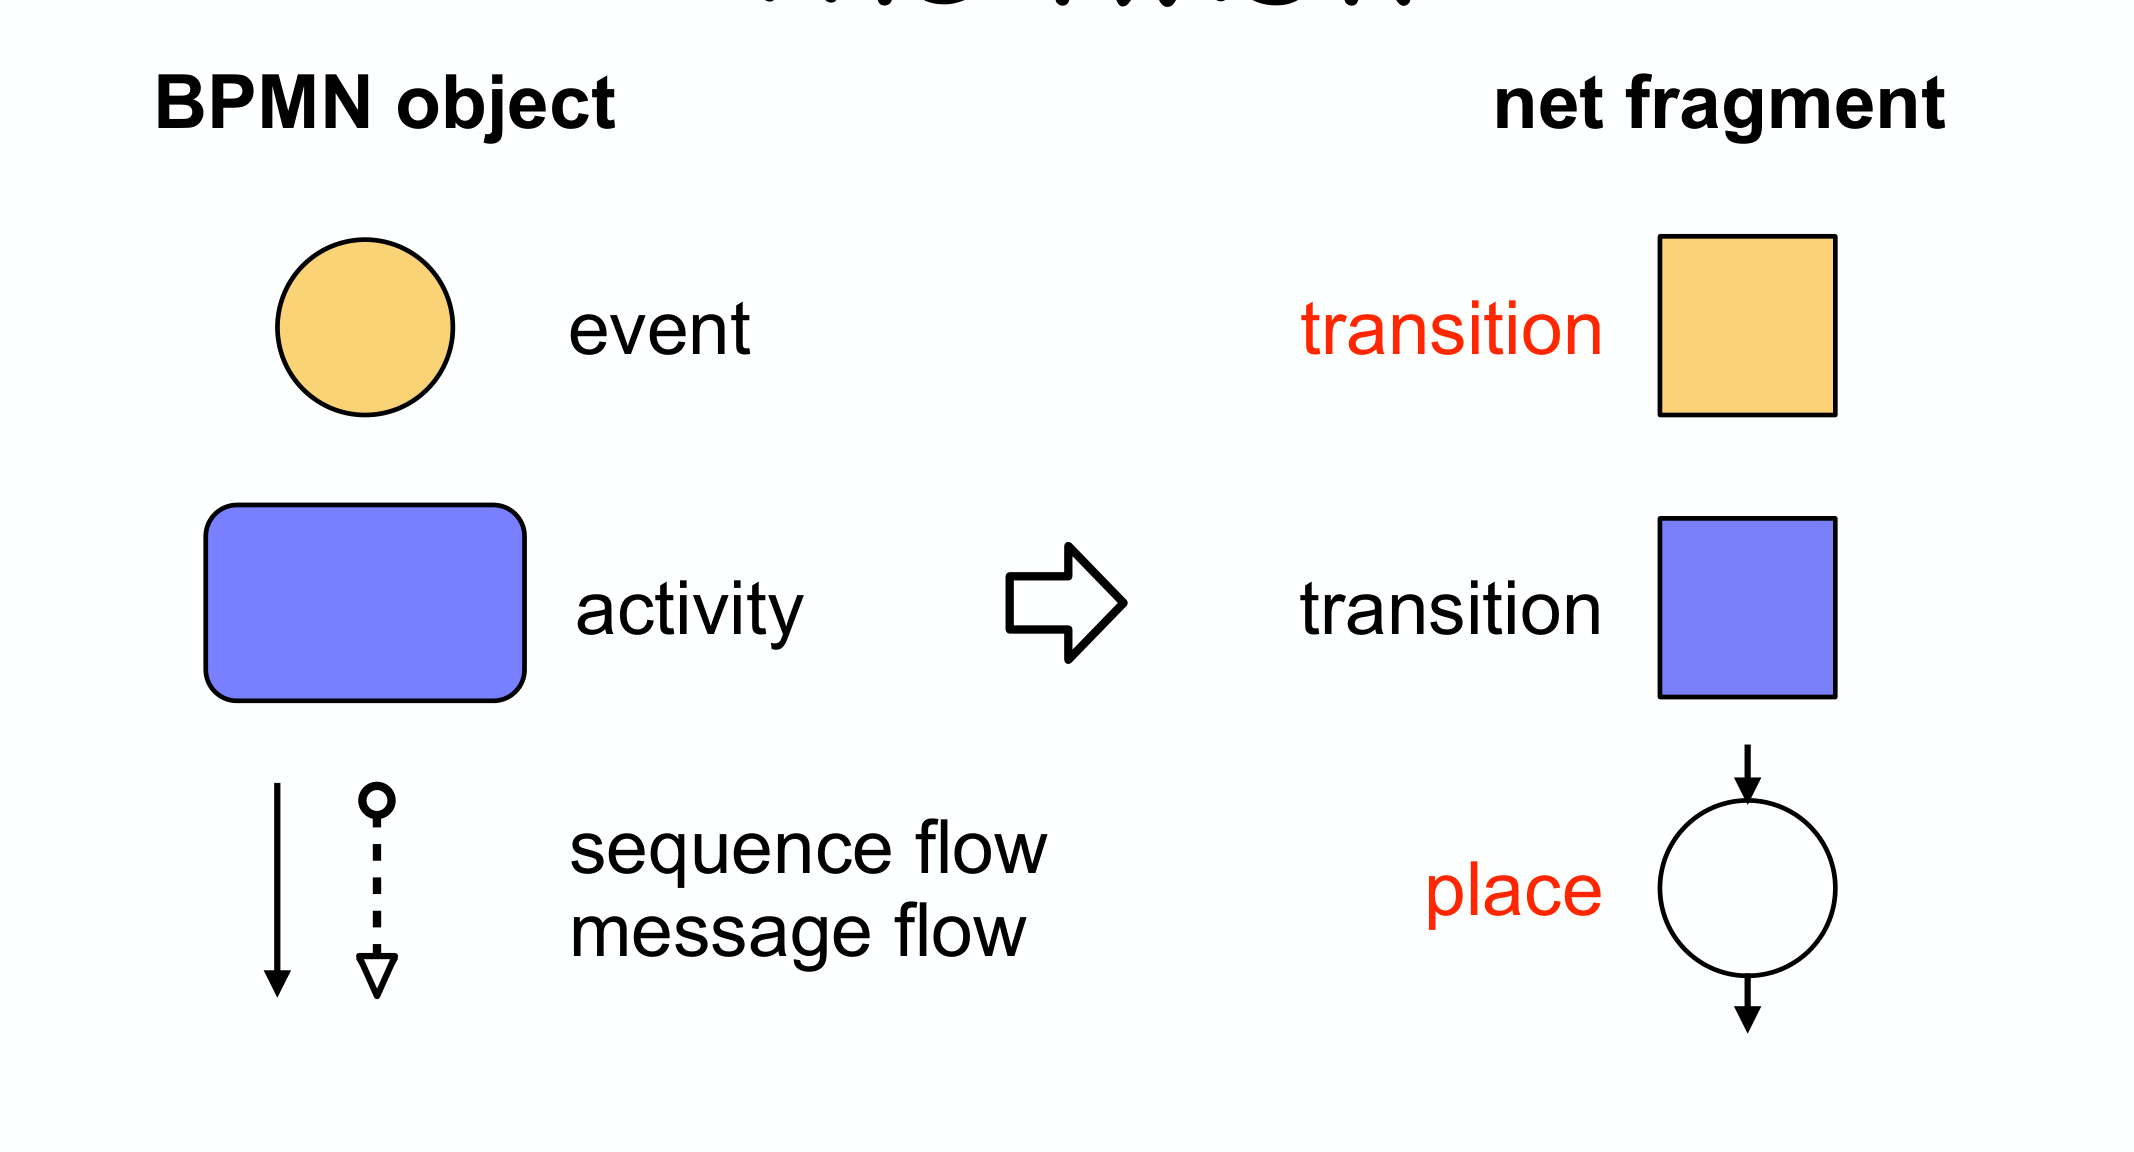
\includegraphics[width=0.74\linewidth,height=0.34\textheight,keepaspectratio]{images/16b-bpmn-analysis_p17_the-twist.png}
\caption{Il "twist": event \textbf{e} activity diventano \textbf{transition}; sequence flow e message flow diventano \textbf{place}. Opposto alla convenzione EPC.}
\end{figure}

\begin{boxnote}{In pratica}
\begin{itemize}
\item un \textbf{place} per ogni arco;
\item una \textbf{transition} per ogni event e per ogni activity;
\item \textbf{una o due} transition per ogni gateway;
\item con qualche \textbf{eccezione} (start/end event, event-based gateway, loop, …) e \textbf{senza oggetti dummy} (a differenza degli EPC!).
\end{itemize}
\end{boxnote}

\subsection{\texorpdfstring{La traduzione in tre step}{La traduzione in tre step}}

\begin{boxnote}{Strategia (3 step)}
\begin{enumerate}
\item \textbf{Step 1 — flussi}: si inserisce un \textbf{place} per ogni sequence flow e message flow.
\item \textbf{Step 2 — flow object}: si inseriscono le \textbf{transition} per event, activity e gateway.
\item \textbf{Step 3 — unico start / unico end}: si forza un solo place iniziale e un solo place finale (con un gateway XOR per lo start; XOR — talvolta AND — per l'end).
\end{enumerate}
\end{boxnote}

I gateway si traducono così:

\begin{figure}[!htb]
\centering
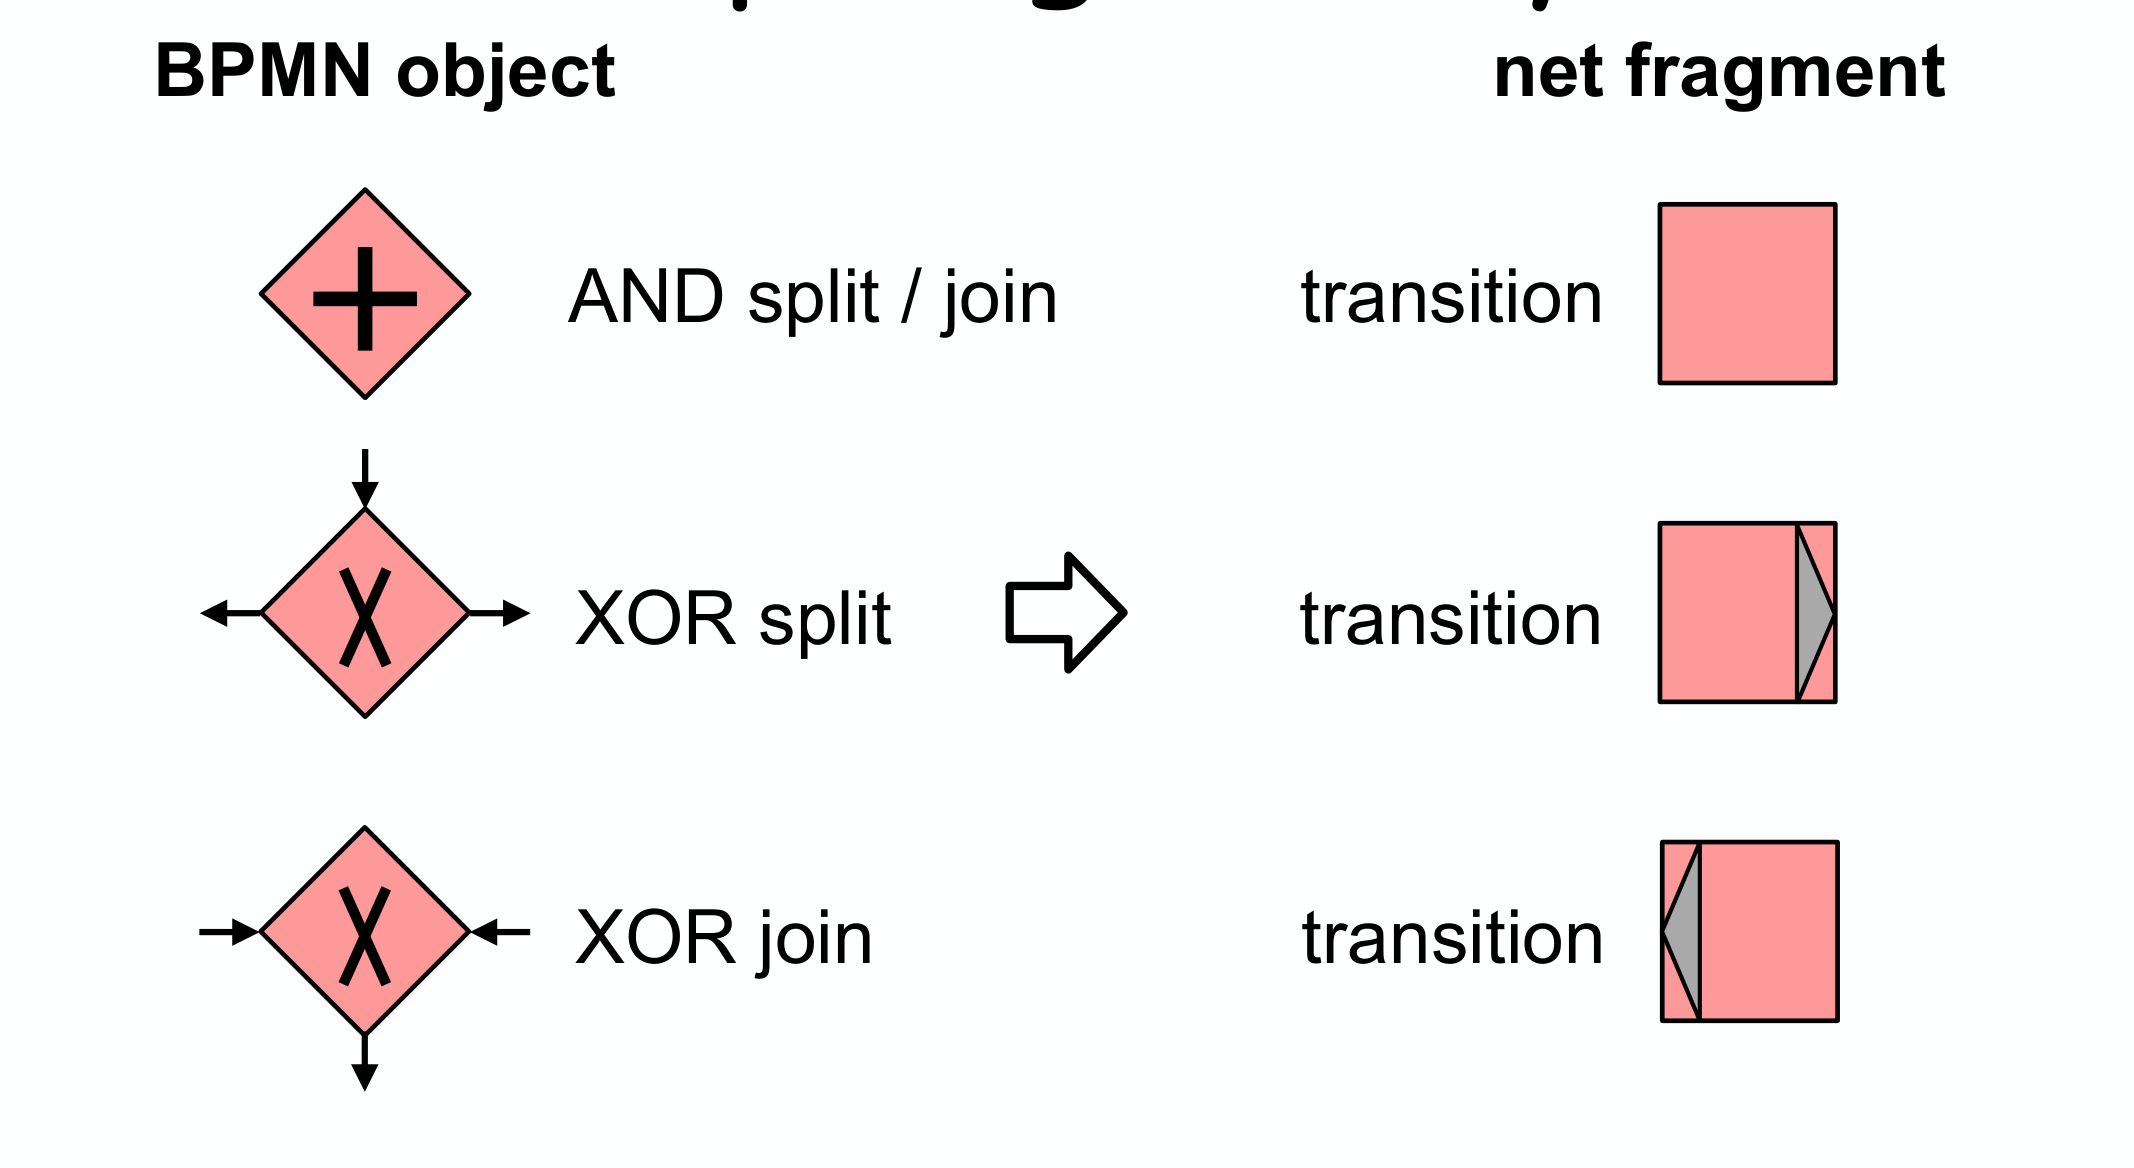
\includegraphics[width=0.74\linewidth,height=0.34\textheight,keepaspectratio]{images/16b-bpmn-analysis_p22_gateways.png}
\caption{I gateway: \textbf{AND split/join} $\rightarrow$ una singola transition (sincronizza/dirama tutti i rami); \textbf{XOR split} e \textbf{XOR join} $\rightarrow$ transition che realizzano la scelta esclusiva. L'\textbf{event-based gateway} si tratta invece con una \textbf{place fusion}.}
\end{figure}

\section{\texorpdfstring{Esempi di analisi}{Esempi di analisi}}

Il bello del metodo è che, tradotto il diagramma, la soundness si legge sul net. Vediamo qualche caso.

\subsection{\texorpdfstring{Order process — non sound}{Order process — non sound}}

\begin{figure}[!htb]
\centering
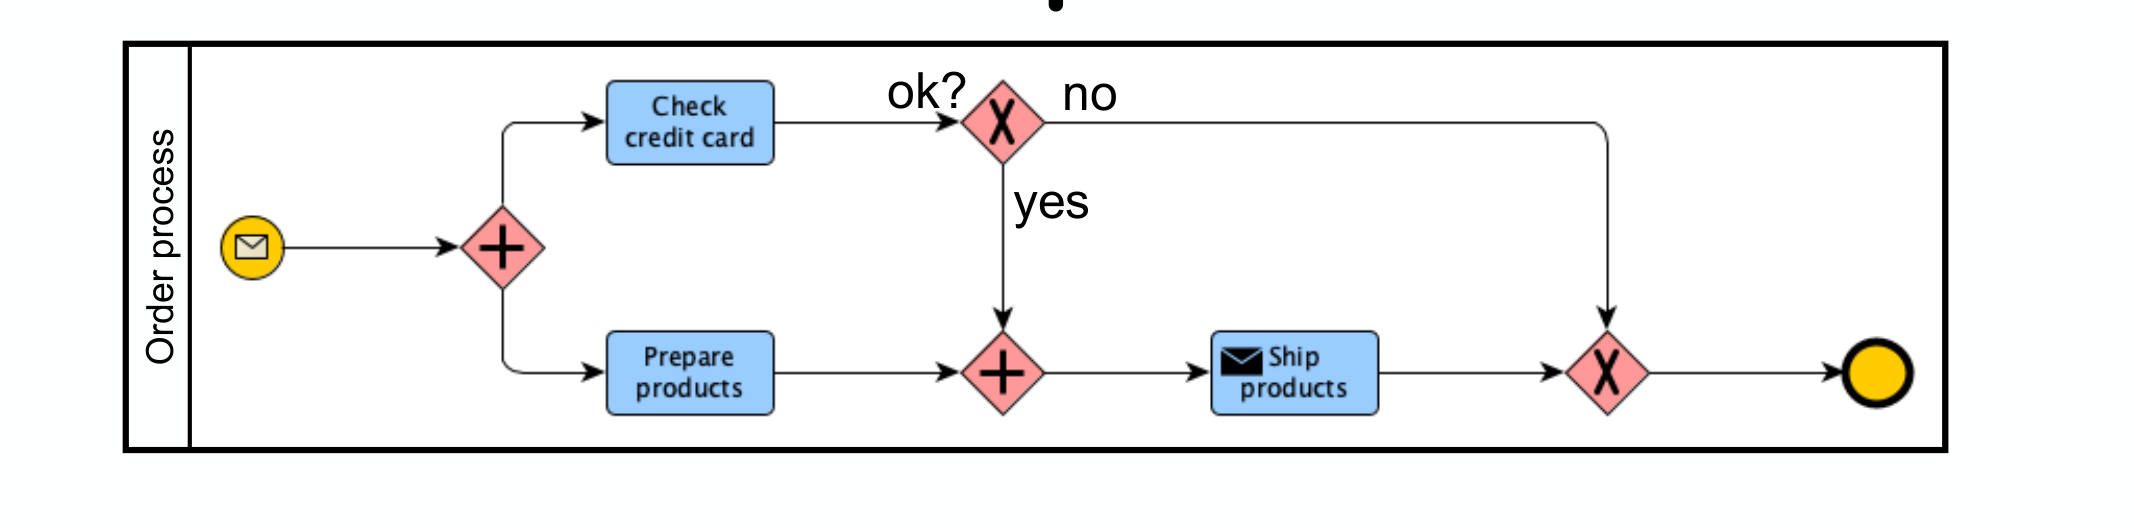
\includegraphics[width=0.74\linewidth,height=0.34\textheight,keepaspectratio]{images/16b-bpmn-analysis_p27_order-process.png}
\caption{Order process. Un \textbf{AND split} avvia in parallelo "check credit card" e "prepare products"; poi uno \textbf{XOR} decide ok?/no.}
\end{figure}

Questo diagramma \textbf{non è sound}. Il difetto è il classico \textbf{mismatch AND/XOR}: l'AND split lancia \emph{due} rami paralleli, ma il ramo "no" dello XOR salta direttamente alla fine \textbf{senza sincronizzare} con l'altro ramo. Risultato: o restano token pendenti (proper completion violata) o si crea un deadlock all'AND join. La combinazione "split di un tipo, join di un altro" è la sorgente di errori più comune nei diagrammi di flusso.

\subsection{\texorpdfstring{Sushi lover / Sushi doomed — sound perché S-net}{Sushi lover / Sushi doomed — sound perché S-net}}

Due process singoli, "Sushi lover" e "Sushi doomed", risultano invece \textbf{safe \& sound}. La ragione è elegante e collega tutto il percorso sui net: le loro traduzioni sono \textbf{S-net} (ogni transition ha un input e un output place). E come sappiamo da \hyperref[ch:15]{15 — S-T Systems}, \textbf{ogni workflow net che sia un S-net è automaticamente safe e sound} — un solo token che scorre, nessuna sincronizzazione da sbagliare.

\subsection{\texorpdfstring{Sushi system — la collaboration}{Sushi system — la collaboration}}

\begin{figure}[!htb]
\centering
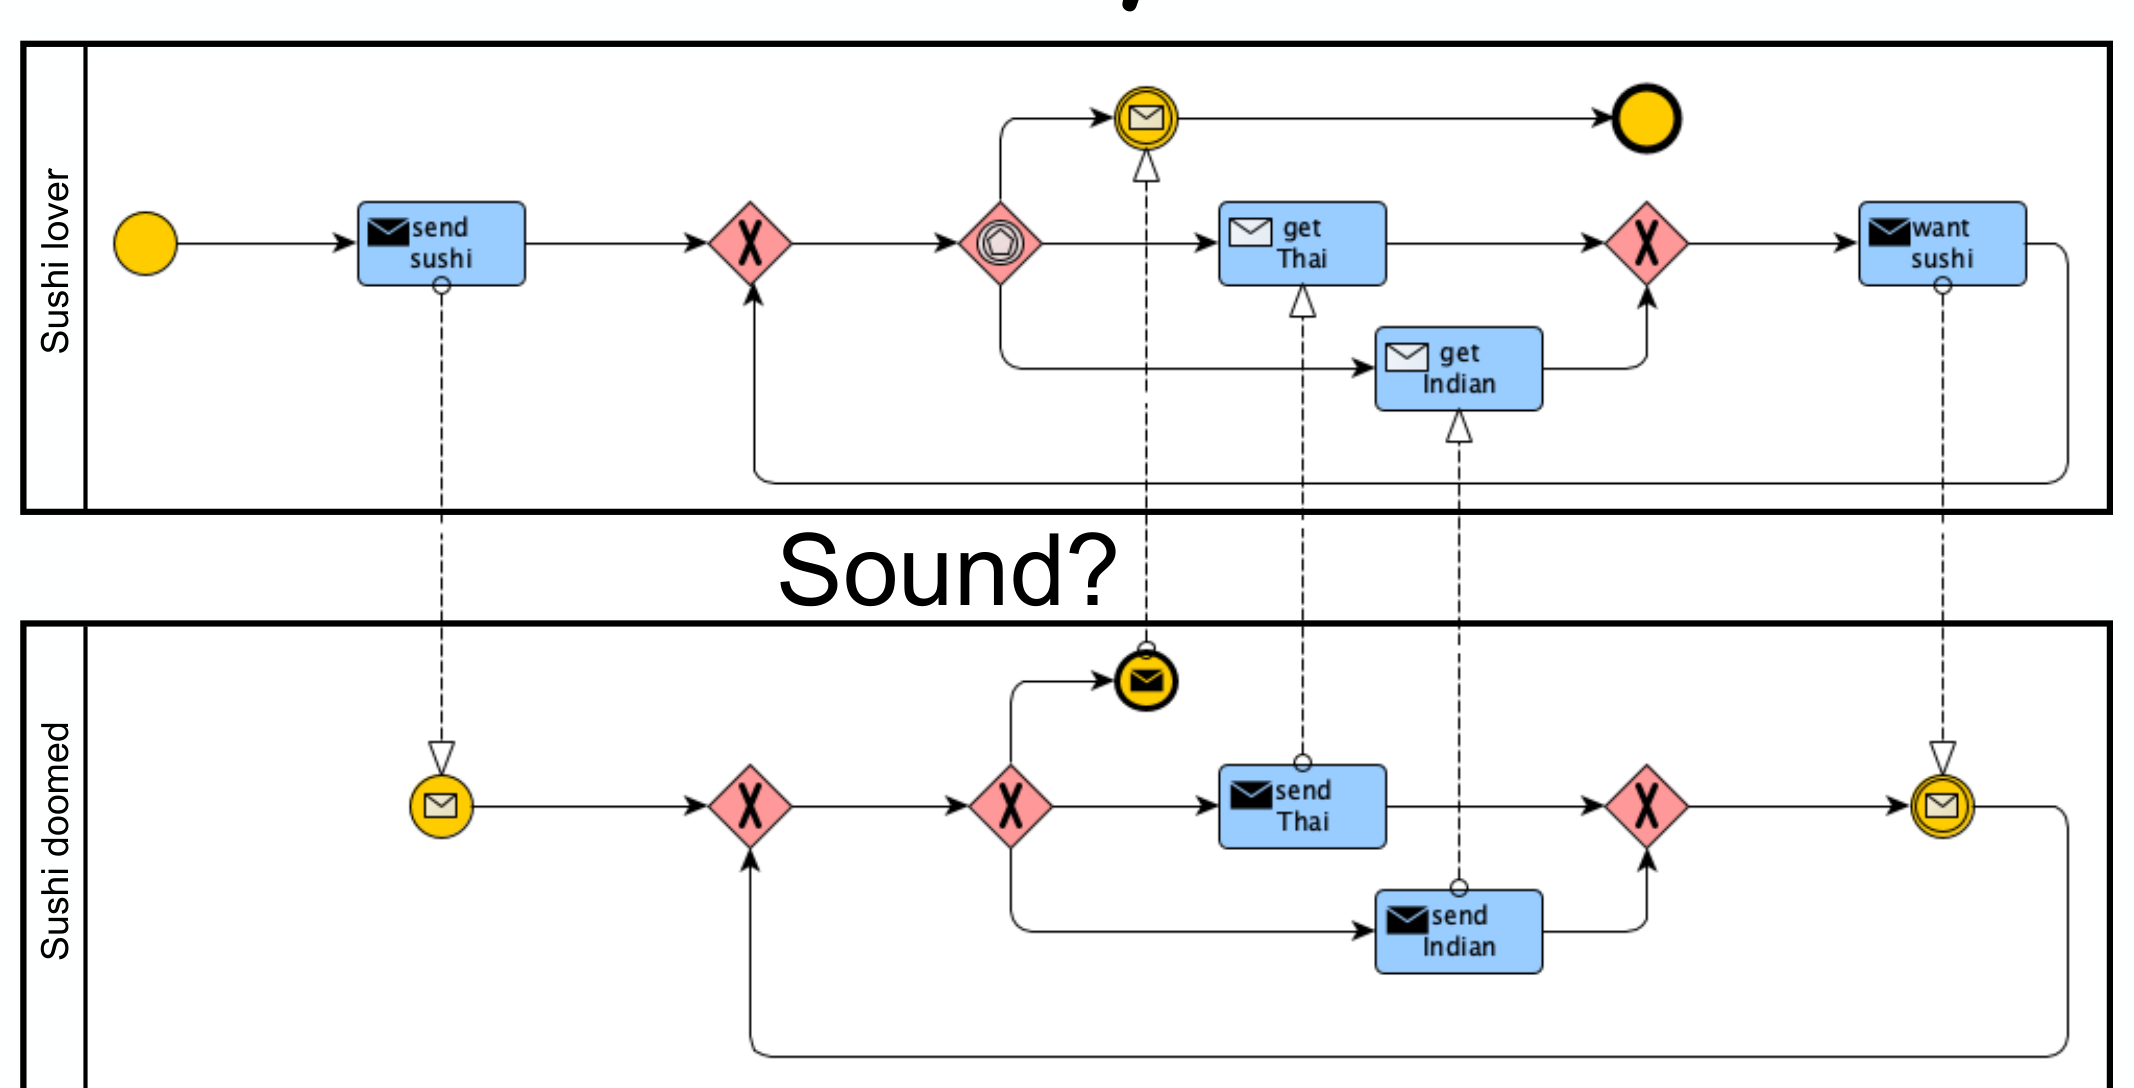
\includegraphics[width=0.74\linewidth,height=0.34\textheight,keepaspectratio]{images/16b-bpmn-analysis_p58_sushi-system.png}
\caption{Sushi system: la \textbf{collaboration} dei due process, che si scambiano messaggi (frecce tratteggiate). Ciascun pool diventa un workflow net; il tutto è un \textbf{workflow system}.}
\end{figure}

Mettendo insieme i due partecipanti in una \textbf{collaboration} (i message flow diventano place condivisi), si ottiene un \textbf{workflow system}. In questo caso l'analisi dice: \textbf{sound!} I due process comunicano in modo coerente.

\subsection{\texorpdfstring{Buyer / Reseller — la sorpresa: sound + sound $\neq$ sound}{Buyer / Reseller — la sorpresa: sound + sound $\neq$ sound}}

\begin{figure}[!htb]
\centering
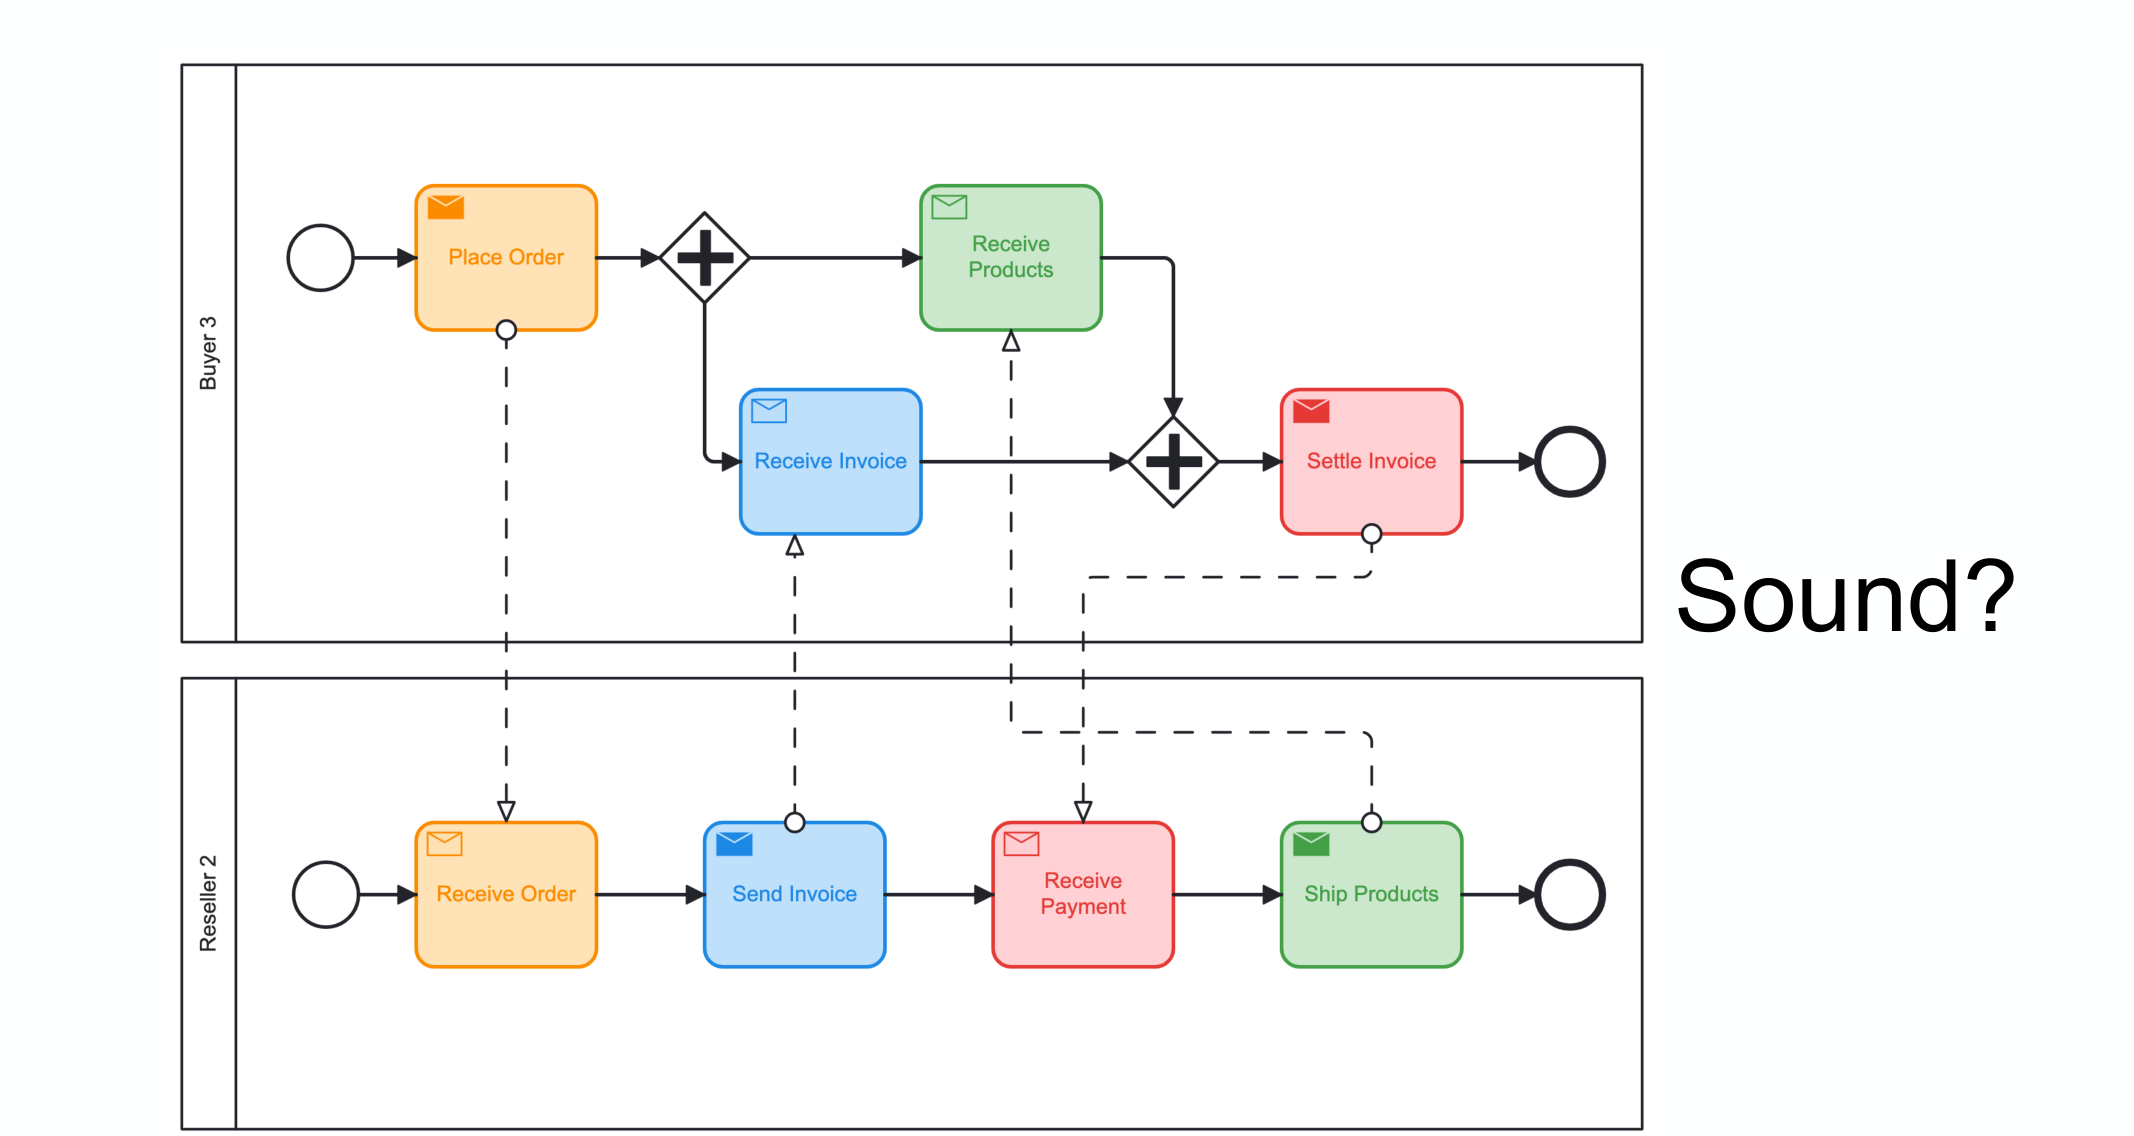
\includegraphics[width=0.74\linewidth,height=0.34\textheight,keepaspectratio]{images/16b-bpmn-analysis_p64_buyer-reseller.png}
\caption{Buyer 3 e Reseller 2. Presi \textbf{singolarmente}, entrambi i process sono \textbf{safe \& sound}. Ma la loro \textbf{collaboration} è… ?}
\end{figure}

Questo è il messaggio più importante della lezione. Presi da soli:

\begin{itemize}
\item \textbf{Buyer 3} $\rightarrow$ safe \& sound;
\item \textbf{Reseller 2} $\rightarrow$ safe \& sound.
\end{itemize}

Ma la loro \textbf{collaboration} (Buyer 3 + Reseller 2) è \textbf{NON sound}! I due partner, corretti individualmente, si bloccano a vicenda quando devono coordinarsi via messaggi — tipicamente una \textbf{dipendenza circolare} fra gli scambi (ciascuno aspetta un messaggio che l'altro invierà solo dopo aver ricevuto il primo).

\begin{boxwarning}{La soundness non composizionale}
La composizione di process \textbf{sound} può dare un system \textbf{non sound}. La correttezza dei singoli partecipanti \textbf{non garantisce} la correttezza della loro collaboration: la comunicazione introduce nuove possibilità di deadlock. Verificare i pezzi separatamente \textbf{non basta} — va analizzato il \textbf{sistema completo}.
\end{boxwarning}

\section{\texorpdfstring{Preprocessing e costrutti avanzati}{Preprocessing e costrutti avanzati}}

Prima della traduzione, alcuni costrutti BPMN richiedono un \textbf{Step 0} di preprocessing, perché non hanno una resa diretta come net "piatto":

\begin{boxnote}{Costrutti che richiedono preprocessing}
\begin{itemize}
\item \textbf{activity looping} (un'attività ripetuta);
\item \textbf{multiple instances} (istanze multiple, limitate a design-time perché il net deve restare finito);
\item \textbf{sub-process} (annidamento);
\item \textbf{exception handling}, su singolo task o su sub-process (l'exception handling su sub-process serve a gestire l'esecuzione separata di più istanze).
\end{itemize}
\end{boxnote}

Questi costrutti si "srotolano" in frammenti di net equivalenti prima di applicare i tre step standard.

\section{\texorpdfstring{Il messaggio finale}{Il messaggio finale}}

Il BPMN, come gli EPC, guadagna una semantica precisa solo pagando un prezzo: si semplifica il diagramma, si evitano gli OR-gateway, e si accetta che la traduzione richieda un "twist" non intuitivo (event e activity $\rightarrow$ transition, archi $\rightarrow$ place). Due lezioni chiave:

\begin{itemize}
\item la \textbf{soundness} dei singoli process spesso si ottiene "gratis" quando la traduzione è un \textbf{S-net} (un solo token che scorre);
\item per le \textbf{collaboration} non vale la composizionalità: \textbf{sound + sound $\neq$ sound}, e va analizzato il workflow system completo.
\end{itemize}

Nella prossima lezione approfondiamo la classe di net che è emersa da queste traduzioni — i \textbf{free-choice net} — e le loro proprietà strutturali. $\rightarrow$ \hyperref[ch:17]{17 — Free Choice}